\chapter{Safe and Near Optimal Controller Synthesis for Stochastic hybrid Games}
  \label{ch:proposal} % In this part goes algorithm, case study and results
  In this part, we propose as case study a \ac{SWH}, modelled as 
  \ac{SHG}, applying the following procedure:
  \emph{System modelling} using physics criteria \cite{tsilingiris1996solar} and
  mechanical concepts to have a \ac{SHG}. Some engineering 
  assumptions either in the model or
  the configuration parameters are considered to facilate our analysis.
  A fundamental characteristic  of the model is the incorporation 
  of uncontrollable events(perturbations) for instance the opening/closing of the valve.
  Secondly, our system interact with a physical environment, for this reason 
  we set some paremeters to get the environment conditions so as 
  understand the temporal data such as \emph{Irradiance}, \emph{external and 
  internal temperatures}, these disturbances are preprocessed to interact
  with our simulator that use \ac{MPC} to control the real-time system 
  using strategies provided by optimizations methods \autoref{sec:casestudy}. 
  To establish a safe sthocastic hybrid game model, we start to compute patterns as
  \autoref{sec:safepatterncomputation} explains. It is important to bear in mind
  the uncontrollable events in our patterns computation to verify the safety
  in our system.
  Lastly, the computation of a near optimal controller consist of an 
  exhaustive exploration of different strategies in order to either
  minimize or maximize a cost function of a random variable in a 
  specific horizon and a model as a stochastic hybrid game, this 
  computation use \textsc{uppaal stratego}. In control experiments 
  we found that this methodology help to concatenate the two 
  approaches implementing a toolbox for a real time simulation in 
  \textsc{python} \cite{larsen2016online}.
  \clearpage
  \section{Solar Water Heating Case study}
    \label{sec:casestudy}
    Solar water heating (SWH) has a widely usage and applications in 
    both domestic and industrial sectors. Solar water heating is not only 
    environment friendly but requires minimal maintenance and operation 
    cost compared to other solar energy \cite{shukla2013recent}. Extensive
    research has been performed to further improve the thermal efficency of
    \ac{SWH}. This research presents a detailed review exclusively
    on the system modelling as stochastic hybrid game and a new way to improve
    the performance, these improvements are not provided from a colector design 
    but from the system behaviour that automaticsally derived a mode of operations 
    with this purpose. \\
    \begin{figure}[!hbt]
      \centering
      

\tikzset{every picture/.style={line width=0.75pt}} %set default line width to 0.75pt        

\begin{tikzpicture}[x=0.75pt,y=0.75pt,yscale=-1,xscale=1]
%uncomment if require: \path (0,300); %set diagram left start at 0, and has height of 300

%Rounded Rect [id:dp3454362135099034] 
\draw   (203,113.4) .. controls (203,105.45) and (209.45,99) .. (217.4,99) -- (282.1,99) .. controls (290.05,99) and (296.5,105.45) .. (296.5,113.4) -- (296.5,156.6) .. controls (296.5,164.55) and (290.05,171) .. (282.1,171) -- (217.4,171) .. controls (209.45,171) and (203,164.55) .. (203,156.6) -- cycle ;
%Straight Lines [id:da8670184653139519] 
\draw    (232.5,128) -- (175.5,128.97) ;
\draw [shift={(173.5,129)}, rotate = 359.03] [color={rgb, 255:red, 0; green, 0; blue, 0 }  ][line width=0.75]    (10.93,-3.29) .. controls (6.95,-1.4) and (3.31,-0.3) .. (0,0) .. controls (3.31,0.3) and (6.95,1.4) .. (10.93,3.29)   ;
%Image [id:dp1573774251550818] 
\draw (329.75,151.88) node  {\includegraphics[width=391.13pt,height=232.5pt]{content/sources/5.png}};
%Straight Lines [id:da756821456781489] 
\draw    (368.5,118.55) -- (450.5,117.57) ;
\draw [shift={(452.5,117.55)}, rotate = 539.3199999999999] [color={rgb, 255:red, 0; green, 0; blue, 0 }  ][line width=0.75]    (10.93,-3.29) .. controls (6.95,-1.4) and (3.31,-0.3) .. (0,0) .. controls (3.31,0.3) and (6.95,1.4) .. (10.93,3.29)   ;
%Straight Lines [id:da9580285561891552] 
\draw    (228.5,102.22) -- (302.5,101.24) ;
\draw [shift={(304.5,101.22)}, rotate = 539.25] [color={rgb, 255:red, 0; green, 0; blue, 0 }  ][line width=0.75]    (10.93,-3.29) .. controls (6.95,-1.4) and (3.31,-0.3) .. (0,0) .. controls (3.31,0.3) and (6.95,1.4) .. (10.93,3.29)   ;
%Straight Lines [id:da9281060785864365] 
\draw    (413,77.89) -- (413,107.89) ;
\draw [shift={(413,109.89)}, rotate = 270] [color={rgb, 255:red, 0; green, 0; blue, 0 }  ][line width=0.75]    (10.93,-3.29) .. controls (6.95,-1.4) and (3.31,-0.3) .. (0,0) .. controls (3.31,0.3) and (6.95,1.4) .. (10.93,3.29)   ;
%Straight Lines [id:da47053369422446445] 
\draw    (261.5,79.22) -- (294.5,79.22) ;
\draw [shift={(296.5,79.22)}, rotate = 180] [color={rgb, 255:red, 0; green, 0; blue, 0 }  ][line width=0.75]    (10.93,-3.29) .. controls (6.95,-1.4) and (3.31,-0.3) .. (0,0) .. controls (3.31,0.3) and (6.95,1.4) .. (10.93,3.29)   ;
%Shape: Circle [id:dp11314595015500317] 
\draw  [color={rgb, 255:red, 0; green, 0; blue, 0 }  ,draw opacity=1 ][fill={rgb, 255:red, 155; green, 155; blue, 155 }  ,fill opacity=1 ] (532.5,92.75) .. controls (532.5,88.19) and (536.19,84.5) .. (540.75,84.5) .. controls (545.31,84.5) and (549,88.19) .. (549,92.75) .. controls (549,97.31) and (545.31,101) .. (540.75,101) .. controls (536.19,101) and (532.5,97.31) .. (532.5,92.75) -- cycle ;
%Shape: Rectangle [id:dp7839106216211671] 
\draw  [color={rgb, 255:red, 0; green, 0; blue, 0 }  ,draw opacity=1 ][fill={rgb, 255:red, 0; green, 0; blue, 0 }  ,fill opacity=0.25 ] (344.33,136.55) -- (352.33,136.55) -- (352.33,174.55) -- (344.33,174.55) -- cycle ;
%Straight Lines [id:da12515710435460292] 
\draw    (375.67,136.55) -- (321,136.22) ;
%Straight Lines [id:da47364591531914657] 
\draw [color={rgb, 255:red, 208; green, 2; blue, 27 }  ,draw opacity=1 ][line width=1.5]    (383,57.89) -- (417,57.89) ;
%Straight Lines [id:da715354649143032] 
\draw  [dash pattern={on 4.5pt off 4.5pt}]  (374.33,104.55) -- (320.33,103.89) ;
%Straight Lines [id:da06846603339970381] 
\draw  [dash pattern={on 4.5pt off 4.5pt}]  (375.67,75.89) -- (321.67,75.22) ;
%Straight Lines [id:da8948879575945841] 
\draw    (340.33,223.89) -- (339.68,147.22) ;
\draw [shift={(339.67,145.22)}, rotate = 449.51] [color={rgb, 255:red, 0; green, 0; blue, 0 }  ][line width=0.75]    (10.93,-3.29) .. controls (6.95,-1.4) and (3.31,-0.3) .. (0,0) .. controls (3.31,0.3) and (6.95,1.4) .. (10.93,3.29)   ;

% Text Node
\draw (455,133) node    {$kA_{t}( T_{c} -T_{e})$};
% Text Node
\draw (193,97) node    {$A_{c} I_{e}$};
% Text Node
\draw (469.33,90) node    {$v\dot{m}( T_{c} -T_{i})$};
% Text Node
\draw (348.33,120) node    {$T_{c} ,V_{c}$};
% Text Node
\draw (568,89) node    {$T_{e}$};
% Text Node
\draw (539,278) node    {$T_{i}$};
% Text Node
\draw (281.33,66.67) node    {$P_{a} =c_{3} r$};
% Text Node
\draw (540,217) node    {$T_{c}$};
% Text Node
\draw (382.67,126.33) node [anchor=north west][inner sep=0.75pt]   [align=left] {1};
% Text Node
\draw (382,93) node [anchor=north west][inner sep=0.75pt]   [align=left] {2};
% Text Node
\draw (382,57.33) node [anchor=north west][inner sep=0.75pt]   [align=left] {3};
% Text Node
\draw (272.67,213.73) node [anchor=north west][inner sep=0.75pt]    {$\frac{dV_{c}( t)}{dt} =pV_{min} -V_{c}( t)$};


\end{tikzpicture}

      \captionsetup{format=hang}
      \caption{Solar Water Heating diagram used to obtain the differential equations}
      \label{fig:casestudy}
    \end{figure} \\
    The system setup is about a hybrid solar water heating which involves 
    Auxiliar energy to heat the system and also a collector that transform 
    solar irradiance to heat energy, transfering it to the container. The system also
    contains a piston which change the volume, in order to simplify the analysis 
    we devide it in three levels as shown in \autoref{fig:casestudy}. We also 
    consider some asumptions in the temperature because of the gradient change
    along the volumen, to facilate the physical modelling we decide to work with 
    the mean temperature as one variable in the state.
    \clearpage 
    \subsection{Data processing and generation}      
      \textbf{Stochastic events as historical data}. In practice
      we notice unpredictable discrete events which can perturbate our dynamical
      system, these stochastic discrete perturbations we call uncontrallable actions and 
      is managed using a stochastic model approach and machine learning to optimize
      the control. To generate these perturbations with a realistic criteria for 
      our case study we choose three gaussian distributions with 
      $\mu_1 = 7h$, $\mu_2 = 12h$ and $\mu_3 = 19h$
      and $\sigma_1=12,\sigma_2=15, \sigma_3=10$ respectively. Finally we add 
      a uniform distribution around the day.
      \begin{figure}[!hbt]      
        \centering
        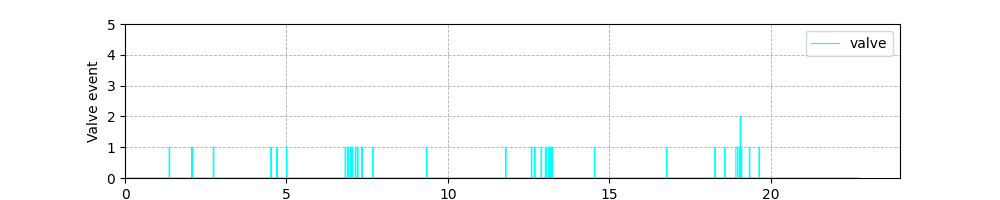
\includegraphics[width=1.2\linewidth]{images/uncontrollable}      
        \captionsetup{format=hang}
        \captionof{figure}{Valves perturbations generated along a day.}
        \label{fig:uncontrollable}
      \end{figure}

      \textbf{Solaris Data and preprocessing} The data collected is from 
      spain solaris, which consist of a set of environment features such as
      environment temperatures and irradiance that would be useful for the 
      simulation. We preprocess the time series data modifying 
      the time step from 15 minutes to 1 minute through interpolation.
      The data is collected from Almeria in Spain \cite{solargis}.

      \begin{figure}[!hbt]
        \centering
        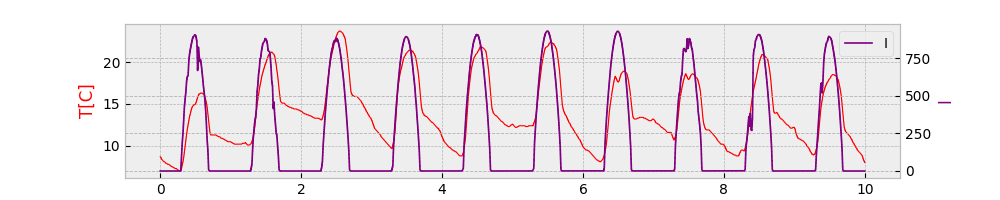
\includegraphics[width=1.2\linewidth]{images/solaris2}
        \captionsetup{format=hang}
        \captionof{figure}{Weather time series, irradiance and temperature }
      \end{figure}
      \clearpage
      
      \textbf{Prediction Data}.
      To integrate a \ac{MPC} in our simulator we configurate
      a forecaster in real time in order to get a sequence of environment data
      on future which will be used to control future states an get the correct
      patterns on present. \textsc{arima} state model is used with a realtime 
      pivot $= 24h$ prediction size $ = 3h$ as shown in \autoref{prediction_environment}, 
      however in the real time simulation we set a prediction size $=1h$ 
       \cite{jain2017study}.

      \begin{minipage}{\linewidth}
        \begin{center}
            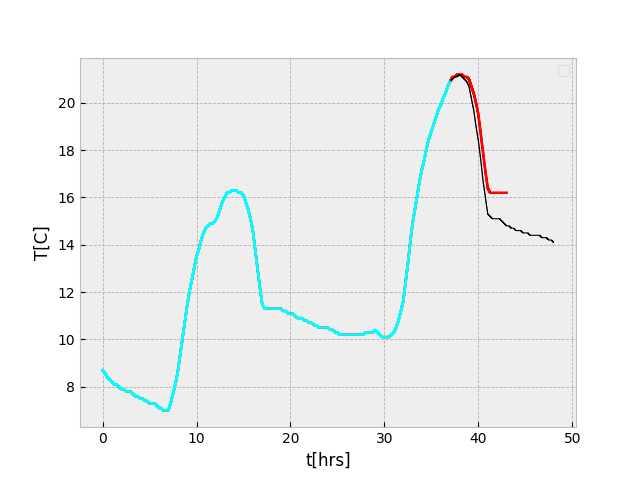
\includegraphics[width=0.7\linewidth]{images/prediction}
            \captionof{figure}{An example of prediction using \textsc{arima} forecaster}
            \label{prediction_environment}
        \end{center}
      \end{minipage}

      Disturbances such as environment temperatures and irradiance affect 
      the system either positive or negative depending of the state and desired state. 
      \emph{Model predictive control} is a method to control establishing in a future 
      horizon to explore best actions control for future states.      
      % \begin{equation} 
      % §    \factorheat\mcont(t)\frac{d}{dt}\tcont =  A_c\irradiance + \haux - v\factorheat \flowin (\tcont-\tin) -   k_c A_t (\tcont-\tenv) + rQ
      %     \label{energy-balance}
      % \end{equation}
      % \begin{equation}
      %     \frac{d}{dt}\mcont(t) =  \rho \frac{d}{dt}\vcont = \rho (pV_{min} - \vcont); \quad
      %     \label{volume-balance}
      % \end{equation}
    % table 
      \begin{table}[hbt!]
      \begin{tabular}{ |p{2cm}||p{6cm}|p{2cm}|p{2cm}|  }
          \hline
          \multicolumn{4}{|c|}{States} \\
          \hline
          Variable& Description &Initial Value&Units\\    
          \hline    
          E & Energy consumption  & 0.0 & \si{\joule} \\
          V & Container Volume  & 0.13 &\si{\metre^3}\\
          T & Container Temperature & 50.0 & \si{\degreeCelsius}  \\            
          \hline
          \multicolumn{4}{|c|}{Constants} \\
          \hline    
          Variable& Description & Value & Units\\        
          \hline
          \factorheat & The factor heat of the water in   & 4186&\si{\joule\per\degreeCelsius\per\kilogram}\\
          \flowin & Mass flow rate input/output  & 0.1  &\si{\kilogram\per\second}\\
          \mcont & the mass of the container in & 100 & \si{\kilogram} \\    
          $A_c$ & Area of colector in & 1 & \si{\metre^2} \\
          $A_t$ & Area of total of surface in & 5.56 & \si{\metre^2} \\
          $k_c$ & Conduction coeficient & 16 & \si{\watt\per\metre\per\degreeCelsius} \\
          $\haux$ & Auxiliary heat power in & 1000 & \si{\watt} \\    
          \hline
          \multicolumn{4}{|c|}{Input values} \\
          \hline    
          Variable& Description &  \multicolumn{2}{|c|}{Space values}\\
          \hline
          $v$ & Controllable action to release water & \multicolumn{2}{|c|}{$\left\lbrace 0,1 \right\rbrace$} \\
          \hline
          $r$ & Controllable action to heat & \multicolumn{2}{|c|}{$\left\lbrace 0,1 \right\rbrace$}\\
          \hline
          $p$ & Uncontrollable action to change capacity water & \multicolumn{2}{|c|}{$\left\lbrace 1,2,3 \right\rbrace$}\\
          \hline         
          \multicolumn{4}{|c|}{Disturbances} \\
          \hline
          Variable& Description & Range&Units\\
          \hline
          $\tin$ & the temperature of water input/output in & $[20-25]$ & \si{\degreeCelsius} \\
          $\irradiance$ & the irradiance in & $[0-920]$ & \si{\watt\per\square\metre}    \\
          $\tenv$ & the outside temperature in & $[0-16.5]$ & \si{\degreeCelsius} \\
          \hline
      \end{tabular}
      \caption{Parameter values used for computing $c_1,c_2, c_3$ and $c_4$.}
      \label{data-table}
      \end{table}
      \clearpage
    \subsection{Hybrid Solar Water Heating as a Sthocastic Hybrid Game}.
      The hybrid solar water heating scenario with 12 modes of operations is
      defined  like this: $\mathcal{G}_{n,m} = (\mathcal{C,U,X,F},\delta)$, 
      where the controller $\mathcal{C}$ has a finite set of controllable actions,
      given by resistance state ${r \in \mathbb{B}}$ and piston position $p \in 
      \left\lbrace1,2,3\right\rbrace $. The environment $\mathcal{U}$ has a finite  
      set of stochastic discrete perturbations $v \in \mathbb{B} $, that means the valve state 
      for opening/closing water aperture. We assume that $\mathcal{U}$ given 
      $\delta$ can switch among modes acording to the probabilistic distributions 
      defined in \autoref{fig:uncontrollable} at every period. 
      The state variables in $\mathcal{X}$ are given by $\left\lbrace 
      E,V,T \right\rbrace $, container temperature, energy used and container 
      volumen respectively.

      Given the container temperature and the volume, a controllable 
      actions $r \in \mathbb{B}$ and $p \in \left\lbrace1,2,3\right\rbrace$,
      a stochastic discrete perturbation $v \in \mathbb{B} $ and a 
      time delay $\tau$ \autoref{fig:casestudy}.

      \begin{equation}
        \begin{aligned}
          \frac{d}{dt}\tcont = \frac{1}{V(t)} [ -\constone(\tcont-\tenv)
          - v \consttwo(\tcont-\tin) \\
          - f \constthree(pV_{min} - \vcont)(\tcont-\tin)
          + \constfour\irradiance + 
          r \constfive ]
        \end{aligned}
        \label{eq:temperature-equation}
      \end{equation}

      \begin{equation}
        \frac{d}{dt}\vcont = pV_{min} - \vcont; \quad
        \label{eq:volume-equation}
      \end{equation}

      \begin{equation} 
        \frac{d}{dt}E_{used} = r \constthree ;
        \label{eq:Energy-equation}
      \end{equation}

      In \ref{eq:temperature-equation}, \ref{eq:volume-equation}, 
      \ref{eq:Energy-equation}  we note some constants $\left\lbrace 
      \constone, \consttwo, \constthree, \constfour \right\rbrace $, these
      are computed with the parameteres defined in table \ref{data-table} 
      resulting $\left\lbrace 2.44e^{-5},  4.77e^{-6}, 0.0024, 0.01 \right\rbrace$ 
      respectively. Another important variable to consider is $f \in 
      \lbrace 0,1 \rbrace$,
      this variable affect the term $f\constthree(pV_{min}-\vcont)(\tcont-\tin)$ 
      that measure the energy removed in the system due to the piston 
      expansion when $p \xrightarrow{\tau} p', (p'>p)$ thus $f=1$
      which imply the incoming of cold water at \autoref{eq:temperature-equation}.
      However, if the piston is contracted, that means 
      $p \xrightarrow{\tau} p', p \geqslant p'$ and hence $f=0$,
      in this case there is no temperature changes but rather a loss of 
      energy due to the outgoing water.
      % According to our case study we find some forbidden transisions such as
      % $\gamma_0 \xrightarrow{\tau} \gamma_{2} $,
      % $\gamma_0 \xrightarrow{\tau} \gamma_{3} $, $\gamma_1 \xrightarrow{\tau} \gamma_{2} $,
      % $\gamma_1 \xrightarrow{\tau} \gamma_{3} $ as well as $\gamma_4 \xrightarrow{\tau} \gamma_{6} $,
      % $\gamma_4 \xrightarrow{\tau} \gamma_{7} $, $\gamma_5 \xrightarrow{\tau} \gamma_{6} $,<
      % $\gamma_5 \xrightarrow{\tau} \gamma_{7} $
      \clearpage

      \begin{figure}[!hbt]
        \centering
        

\tikzset{every picture/.style={line width=0.75pt}} %set default line width to 0.75pt        

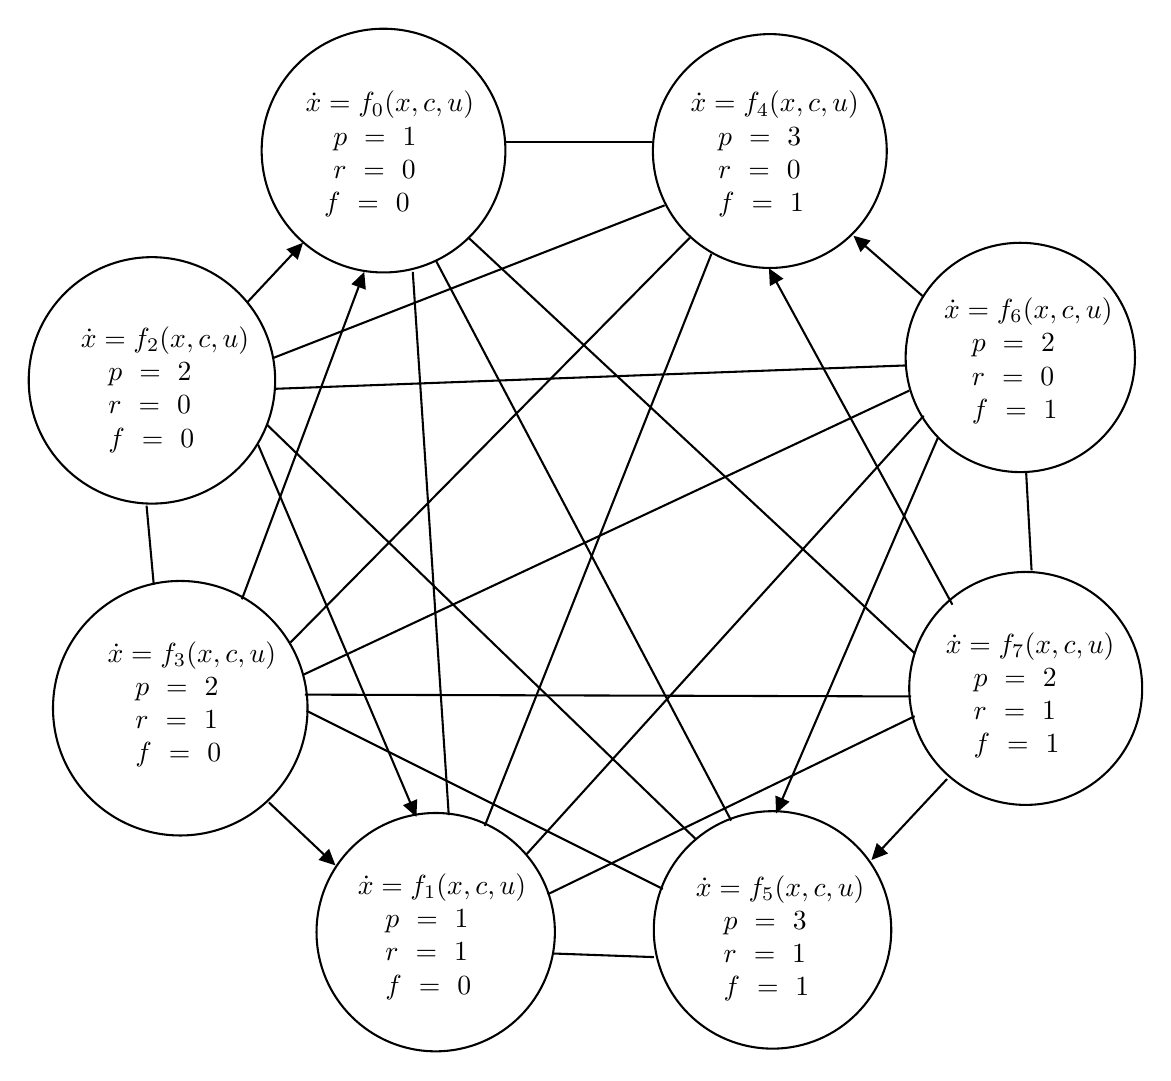
\begin{tikzpicture}[x=0.65pt,y=0.65pt,yscale=-1,xscale=1]
%uncomment if require: \path (0,869); %set diagram left start at 0, and has height of 869

%Shape: Circle [id:dp8105865911695849] 
\draw   (382.5,274.5) .. controls (382.5,236.67) and (413.17,206) .. (451,206) .. controls (488.83,206) and (519.5,236.67) .. (519.5,274.5) .. controls (519.5,312.33) and (488.83,343) .. (451,343) .. controls (413.17,343) and (382.5,312.33) .. (382.5,274.5) -- cycle ;
%Shape: Circle [id:dp4238655727754186] 
\draw   (396,456.75) .. controls (396,417.68) and (427.68,386) .. (466.75,386) .. controls (505.82,386) and (537.5,417.68) .. (537.5,456.75) .. controls (537.5,495.82) and (505.82,527.5) .. (466.75,527.5) .. controls (427.68,527.5) and (396,495.82) .. (396,456.75) -- cycle ;
%Shape: Circle [id:dp2933944994958515] 
\draw   (512,146.75) .. controls (512,109.33) and (542.33,79) .. (579.75,79) .. controls (617.17,79) and (647.5,109.33) .. (647.5,146.75) .. controls (647.5,184.17) and (617.17,214.5) .. (579.75,214.5) .. controls (542.33,214.5) and (512,184.17) .. (512,146.75) -- cycle ;
%Shape: Circle [id:dp9366456554811557] 
\draw   (542.5,581.25) .. controls (542.5,544.66) and (572.16,515) .. (608.75,515) .. controls (645.34,515) and (675,544.66) .. (675,581.25) .. controls (675,617.84) and (645.34,647.5) .. (608.75,647.5) .. controls (572.16,647.5) and (542.5,617.84) .. (542.5,581.25) -- cycle ;
%Shape: Circle [id:dp7320262061476854] 
\draw   (729.5,147) .. controls (729.5,111.1) and (758.6,82) .. (794.5,82) .. controls (830.4,82) and (859.5,111.1) .. (859.5,147) .. controls (859.5,182.9) and (830.4,212) .. (794.5,212) .. controls (758.6,212) and (729.5,182.9) .. (729.5,147) -- cycle ;
%Shape: Circle [id:dp08196792261757313] 
\draw   (730,580) .. controls (730,543.55) and (759.55,514) .. (796,514) .. controls (832.45,514) and (862,543.55) .. (862,580) .. controls (862,616.45) and (832.45,646) .. (796,646) .. controls (759.55,646) and (730,616.45) .. (730,580) -- cycle ;
%Shape: Circle [id:dp2726927054913544] 
\draw   (870,261.75) .. controls (870,226.54) and (898.54,198) .. (933.75,198) .. controls (968.96,198) and (997.5,226.54) .. (997.5,261.75) .. controls (997.5,296.96) and (968.96,325.5) .. (933.75,325.5) .. controls (898.54,325.5) and (870,296.96) .. (870,261.75) -- cycle ;
%Shape: Circle [id:dp447834466431017] 
\draw   (872,445.75) .. controls (872,409.99) and (900.99,381) .. (936.75,381) .. controls (972.51,381) and (1001.5,409.99) .. (1001.5,445.75) .. controls (1001.5,481.51) and (972.51,510.5) .. (936.75,510.5) .. controls (900.99,510.5) and (872,481.51) .. (872,445.75) -- cycle ;
%Straight Lines [id:da771329734195769] 
\draw    (504.01,231.11) -- (532.95,200.19) ;
\draw [shift={(535,198)}, rotate = 493.1] [fill={rgb, 255:red, 0; green, 0; blue, 0 }  ][line width=0.08]  [draw opacity=0] (8.93,-4.29) -- (0,0) -- (8.93,4.29) -- cycle    ;
%Straight Lines [id:da24943983750644705] 
\draw    (647.01,142.11) -- (729.01,142.11) ;
%Straight Lines [id:da9374471528095312] 
\draw    (843.28,196.08) -- (880.01,228.11) ;
\draw [shift={(841.01,194.11)}, rotate = 41.08] [fill={rgb, 255:red, 0; green, 0; blue, 0 }  ][line width=0.08]  [draw opacity=0] (8.93,-4.29) -- (0,0) -- (8.93,4.29) -- cycle    ;
%Straight Lines [id:da20228861715808955] 
\draw    (937.01,326.11) -- (940.01,380.11) ;
%Straight Lines [id:da1309980038885339] 
\draw    (730.01,595.11) -- (674.01,593.11) ;
%Straight Lines [id:da8387653364416086] 
\draw    (893.01,496.11) -- (853.06,538.91) ;
\draw [shift={(851.01,541.11)}, rotate = 313.03] [fill={rgb, 255:red, 0; green, 0; blue, 0 }  ][line width=0.08]  [draw opacity=0] (8.93,-4.29) -- (0,0) -- (8.93,4.29) -- cycle    ;
%Straight Lines [id:da15505665307834682] 
\draw    (550.83,542.05) -- (516.01,509.11) ;
\draw [shift={(553.01,544.11)}, rotate = 223.41] [fill={rgb, 255:red, 0; green, 0; blue, 0 }  ][line width=0.08]  [draw opacity=0] (8.93,-4.29) -- (0,0) -- (8.93,4.29) -- cycle    ;
%Straight Lines [id:da9785106227459619] 
\draw    (452.01,388.11) -- (448.01,344.11) ;
%Straight Lines [id:da40579582190774643] 
\draw    (795.45,214.83) -- (896.01,399.2) ;
\draw [shift={(794.01,212.2)}, rotate = 61.39] [fill={rgb, 255:red, 0; green, 0; blue, 0 }  ][line width=0.08]  [draw opacity=0] (8.93,-4.29) -- (0,0) -- (8.93,4.29) -- cycle    ;
%Straight Lines [id:da9504222588958726] 
\draw    (888.01,306.2) -- (799.2,512.44) ;
\draw [shift={(798.01,515.2)}, rotate = 293.3] [fill={rgb, 255:red, 0; green, 0; blue, 0 }  ][line width=0.08]  [draw opacity=0] (8.93,-4.29) -- (0,0) -- (8.93,4.29) -- cycle    ;
%Straight Lines [id:da4817256852969489] 
\draw    (510.01,310.2) -- (596.84,514.44) ;
\draw [shift={(598.01,517.2)}, rotate = 246.97] [fill={rgb, 255:red, 0; green, 0; blue, 0 }  ][line width=0.08]  [draw opacity=0] (8.93,-4.29) -- (0,0) -- (8.93,4.29) -- cycle    ;
%Straight Lines [id:da5197840649707755] 
\draw    (567.96,217.01) -- (501.01,396.2) ;
\draw [shift={(569.01,214.2)}, rotate = 110.49] [fill={rgb, 255:red, 0; green, 0; blue, 0 }  ][line width=0.08]  [draw opacity=0] (8.93,-4.29) -- (0,0) -- (8.93,4.29) -- cycle    ;
%Straight Lines [id:da6155672485715638] 
\draw    (519.01,279.2) -- (870.01,266.2) ;
%Straight Lines [id:da5361536697962814] 
\draw    (518.01,262.2) -- (736.01,177.2) ;
%Straight Lines [id:da7329803706341473] 
\draw    (536.01,449.2) -- (873.01,450.2) ;
%Straight Lines [id:da47359936905090594] 
\draw    (659.01,538.2) -- (880.01,294.2) ;
%Straight Lines [id:da5004090611197451] 
\draw    (762.01,204.2) -- (636.01,522.2) ;
%Straight Lines [id:da8612879134092823] 
\draw    (596.01,214.2) -- (616.01,516.2) ;
%Straight Lines [id:da26459344362918436] 
\draw    (535.01,438.2) -- (872.01,280.2) ;
%Straight Lines [id:da8834205218815725] 
\draw    (537.01,458.2) -- (735.01,557.2) ;
%Straight Lines [id:da2941468624363204] 
\draw    (528.01,420.2) -- (750.01,195.2) ;
%Straight Lines [id:da9095983178937885] 
\draw    (515.01,299.2) -- (753.01,529.2) ;
%Straight Lines [id:da668275173400011] 
\draw    (627.01,195.2) -- (875.01,426.2) ;
%Straight Lines [id:da943066290095641] 
\draw    (609.01,208.2) -- (773.01,519.2) ;
%Straight Lines [id:da14407547098091467] 
\draw    (671.01,560.2) -- (875.01,461.2) ;

% Text Node
\draw (458.25,280.25) node    {$ \begin{array}{l}
\dot{x} =f_{2}( x,c,u)\\
\ \ \ p\ =\ 2\\
\ \ \ r\ =\ 0\\
\ \ \ f\ =\ 0
\end{array}$};
% Text Node
\draw (473.25,455.25) node    {$ \begin{array}{l}
\dot{x} =f_{3}( x,c,u)\\
\ \ \ p\ =\ 2\\
\ \ \ r\ =\ 1\\
\ \ \ f\ =\ 0
\end{array}$};
% Text Node
\draw (797.25,149.25) node    {$ \begin{array}{l}
\dot{x} =f_{4}( x,c,u)\\
\ \ \ p\ =\ 3\\
\ \ \ r\ =\ 0\\
\ \ \ f\ =\ 1
\end{array}$};
% Text Node
\draw (800.25,585.25) node    {$ \begin{array}{l}
\dot{x} =f_{5}( x,c,u)\\
\ \ \ p\ =\ 3\\
\ \ \ r\ =\ 1\\
\ \ \ f\ =\ 1
\end{array}$};
% Text Node
\draw (583.25,149.25) node    {$ \begin{array}{l}
\dot{x} =f_{0}( x,c,u)\\
\ \ \ p\ =\ 1\\
\ \ \ r\ =\ 0\\
\ \ f\ =\ 0
\end{array}$};
% Text Node
\draw (612.25,584.25) node    {$ \begin{array}{l}
\dot{x} =f_{1}( x,c,u)\\
\ \ \ p\ =\ 1\\
\ \ \ r\ =\ 1\\
\ \ \ f\ =\ 0
\end{array}$};
% Text Node
\draw (938.25,264.25) node    {$ \begin{array}{l}
\dot{x} =f_{6}( x,c,u)\\
\ \ \ p\ =\ 2\\
\ \ \ r\ =\ 0\\
\ \ \ f\ =\ 1
\end{array}$};
% Text Node
\draw (939.25,450.25) node    {$ \begin{array}{l}
\dot{x} =f_{7}( x,c,u)\\
\ \ \ p\ =\ 2\\
\ \ \ r\ =\ 1\ \\
\ \ \ f\ =\ 1
\end{array}$};


\end{tikzpicture}

        \captionsetup{format=hang}
        \caption{Automaton with forbidden transitions because of the addition of a 
        discrete variable \emph{f} which facilate the system modelling either on
        piston expansion or compression, the perturbation of the valve is not considered
        in this representation as discrete state but rather as interval box.}
        \label{fig:automaton}
      \end{figure}
      As we notice, there are eight operation modes, is because in this step
      we do not care the stochasticity  either perturbations or disturbances 
      will be considered as intervals assuming the best and the worst case.
      There are forbidden transitions in the automaton, for this reason we 
      modify the algorithm which not filter forbidden transitions, otherwise
      the algorihtm ignore the direction exploring modes which can cause problems
      in the pattern search.
      % Finally we set as controllable actions $c = (p,r,f) \in \lbrace 1,2,3 \rbrace \times 
      % \lbrace 0,1 \rbrace \times \lbrace 0,1 \rbrace $ and uncontrollable actions 
      % \hlc{ $u = \sum_{i=0}^{3} p_{i}(t)$, $p_1(t)$ }as shown at \autoref{fig:uncontrollable}.      
      \clearpage 
      \
      \
      \begin{figure}
      % \begin{algorithm}
        % \caption{Find Pattern with forbidden transitions}\label{euclid}
        \begin{algorithmic}[1]
          \Procedure{FindPattern}{$W,R,S,B,K$}\Comment{List of set of patterns} \\
            \textbf{Input:} A box $W$, a box $R$,
            a box $S$, a box $B$, a length $K$ of input pattern\\
            \textbf{Output:} $<\prod,True> or <_,False>$ \\
            $\mathcal{S}= \lbrace \emptyset \rbrace$ \\
            $\mathcal{L}= \lbrace (W,W,\emptyset) \rbrace$
            \While{$\mathcal{L} \neq \emptyset$}
              \State $e_{current} = takeHead(\mathcal{L})$
              \For{$i \in U$}:
                \If {$Pair(l,i) = False $}\Comment{$l$ is the current mode}
                  \State \textbf{continue}\Comment{Not considered transition $l,i$}
                \EndIf
                \label{alg:filter_transitions}
                \If {$ Post_{i}(e_{current}.Y_{current}) \subseteq R$ \textbf{and} $Tube_{i}(e_{current}.Y_{current}) \cup B = \emptyset $ \textbf{and} $Tube_{i}(e_{current}.Y_{current}) \cup B \subseteq S $ }
                  \State putTail($\mathcal{S}e_{current}.\prod + i$)
                \Else
                  \If{$ Tube_{i}(e_{current}.Y_{current}) \cap B \neq \emptyset $ \textbf{or} $ Tube_{i}(e_{current}.Y_{current}) \nsubseteq S $}
                    \State discard $e_{current}$
                  \EndIf
                  \If{$ Tube_{i}(e_{current}.Y_{current}) \cap B = \emptyset $ \textbf{and} $ Tube_{i}(e_{current}.Y_{current}) \subseteq S $}
                    \If {$Length(\prod)+1<K$}
                      \State putTail$(\mathcal{L},(e_{current}.Y_{init}.Post_{i}(e_{current}.Y_{current}),e_{current}.\prod+i))$
                    \EndIf              
                  \EndIf
                \EndIf
              \EndFor          
            \EndWhile
            \State \textbf{return} $<_,False>$ \Comment{if no solution is found, or $<\prod,True>$, $\prod$ beaing any pattern validated in $Solution$.}
          \EndProcedure    
        \end{algorithmic}
        \captionsetup{format=hang}
        \caption{This algorithm is modified to ignore forbidden transitions  
        and is improved filtering invalid transition in the line 9.}
      % \end{algorithm}
      \end{figure}                  
      % This algorithm is modified to ignore forbidden transitions  and studied in 
      % \cite{le2017improved} is improved filtering invalid transition in the line \ref{alg:filter_transitions}.
      \clearpage

  \section{Experiments: }
    \subsection{Patterns computation}
      To establish a safe stochastic hybrid game,
      we start to compute patterns as the \autoref{sec:safepatterncomputation} 
      explains. It is important to bear in mind that the stochastic discrete
      perturbation $v$ is considered as an interval $[0,1]$, thus in the second term
      in the \autoref{eq:temperature-equation} results $Interval(0,1)c_2(x[0]-Ti)/(0.1p)$,
      which means the term becomes zero when the valve is close. However, 
      when the valve is open the term will change to its biggest value due to
      the cold water incoming and warm water outgoing. Safe patterns are 
      computed and associated to zonotopes,which are regions where patterns
      verify the next: Given $D = 20, K = 3$ and by constructing a law 
      $\sigma$, such that for all $x_o \in R$, and under the unknown 
      bounded perturbation $d$, there exists a $ \sigma: \mathbb{C} \rightarrow C^k$ for      
      some $k$ such that:      
      Such a law permits to perform a safe control guaranteeing limits for each
      action in each step conditioning a safe sequence of modes called 
      \emph{pattern} which verify stability and safety defined in
       \autoref{sec:safepatterncomputation}.

      % \begin{figure}[!hbt]
      %   \begin{center}
      %       

\tikzset{every picture/.style={line width=0.75pt}} %set default line width to 0.75pt        

\begin{tikzpicture}[x=0.75pt,y=0.75pt,yscale=-1,xscale=1]
%uncomment if require: \path (0,310); %set diagram left start at 0, and has height of 310

%Image [id:dp5662256713421685] 
\draw (319,152) node  {\includegraphics[width=274.5pt,height=246pt]{content/sources/safe_post_pattern.png}};

% Text Node
\draw (218,194) node [anchor=north west][inner sep=0.75pt]   [align=left] {$\displaystyle R$};
% Text Node
\draw (206,240) node [anchor=north west][inner sep=0.75pt]   [align=left] {$\displaystyle S$};
% Text Node
\draw (335,150) node [anchor=north west][inner sep=0.75pt]   [align=left] {$\pi _{1} =( 1,3,0)$};
% Text Node
\draw (381,71) node [anchor=north west][inner sep=0.75pt]   [align=left] {$\pi _{2} =( 5,0)$};
% Text Node
\draw (228,96) node [anchor=north west][inner sep=0.75pt]   [align=left] {$\pi _{3} =( 4,0)$};

\end{tikzpicture}

      %       \captionsetup{format=hang}
      %       \caption{Simulation for the first three patterns}
      %       \label{fig:patternsimulation}
      %   \end{center}
      % \end{figure}

      \begin{figure}[!htb]        
        \begin{subfigure}{0.51\textwidth}
          \includegraphics[width=1.0\linewidth]{images/safe_post_pattern.png}
          \captionsetup{format=hang}
          \caption{Simulation for the first three patterns of lengths $3,2,3$ respectively.} 
          \label{fig:safepostpattern}
        \end{subfigure}
        \hspace*{\fill}
        \begin{subfigure}{0.51\textwidth}
          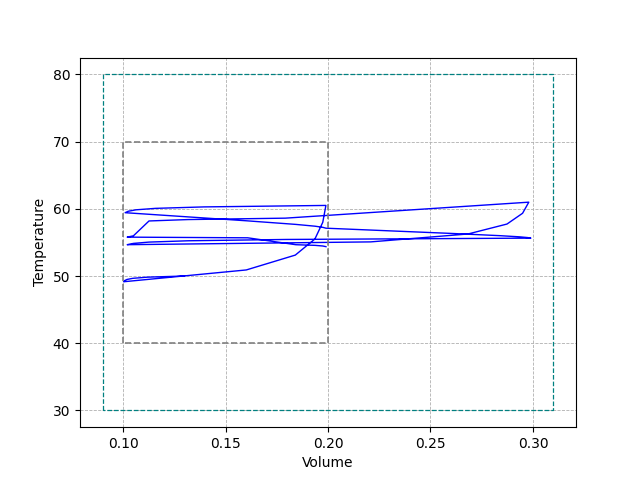
\includegraphics[width=1.0\linewidth]{images/safe_post_pattern_perturb.png}
          \captionsetup{format=hang}
          \caption{Stabilization after the normal perturbation $u=7h,\sigma=1.6$ between $6h$ and $8h$.} 
          \label{fig:safepostpatternperturbation}
        \end{subfigure}%                  
      \end{figure}

      We define the boundaries for the \ac{SWH} such as 
      $R = \begin{bmatrix} 40 & 70 \\ 0.1 & 0.2
      \end{bmatrix}$, $S = \begin{bmatrix} 30 & 80 \\ 0.09 & 0.31 \end{bmatrix}$,
      $W = \begin{bmatrix} 40 & 70 \\ 0.1 & 0.2 \end{bmatrix}$,
      $B = \begin{bmatrix} 0 & 0 \\ 0 & 0 \end{bmatrix}$ that are required for the 
      decomposition algorithm developed in \cite{liberzon2003switching}. We can 
      see the states returning to the $R$ region after finish the pattern 
      satisfying stability and safety in the simulation \autoref{fig:safepostpattern}.
      However, the algorithm is able to stabilize even when a perturbation 
      occur as \autoref{fig:safepostpatternperturbation}.
      \clearpage        
    \subsection{Real Time Model Predictive Controller}
      \textsc{python simulator}. We implement a \emph{toolbox} which incorporate
      sthocastic hybrid models $\mathcal{G}_{n,m}$ and controllers $\mathcal{C}$.
      The models works with seasonal data  \emph{disturbances} for this reason we 
      incorporate modules to preprocess the data. In the initial step of the model 
      predictive algorithm to control \ac{MPC}. The application of \ac{MPC} to 
      stochastic hybrid games subject to disturbances and
      stochastic perturbations gives rise to uncertain optimization problems.
      We use the first pattern corresponding to the current zonotope. In the subsequent 
      iterations we use the \textsc{stratego} to find a near optimal strategy from a selected
      set of safe patterns as show \ref{sssection:upppalstratego}. It is very important to bear in mind 
      the way of model predictive controler operate which is an asynchrnous call 
      before finish the last mode in the current pattern, sending to \textsc{stratego}
      the current dynamical states such as \emph{mode, volume, temperature} and so on with the
      corresponding environment predictions \ref{prediction_environment}.
      After the near optimal pattern computation for stochastic hybrid game 
      by \textsc{stratego} the process repeat.

    \subsection{Controllers Optimizations:}
      Regarding our experiments, we implement two controller synthesis 
      optimization over a real time simulator which run a \ac{MPC} and 
      synthetize a switching rule $\sigma$ written in  \textsc{Python} 
      and a number of controllers associated to two optimization, 
      including a greedy method and the ones produced by \textsc{uppaal 
      stratego}. The simulator use our case study a \ac{SWH} as plant
      and a \ac{SHG} $\mathcal{G}_{n,m}$ as model in the second 
      optimization. We introduce the optimizations which we use in our experiments. We
      present the current controller operating in the house, one controller
      proposed by engineers and another one controller synthetized using 
      online synthesis and \textsc{uppaal-stratego} as follows.

      \subsubsection{ \emph{Greedy optimization}}
        The greddy controller explore a set of patterns that correspond to the 
        current zonotope and is chosen the pattern that minimize
        the cost function. Due to the use of a complete pattern, this 
        approach is able to guaranteeing a safe behaviour. Additionally, this 
        approach only optimize partially due to the stochasticity is ignored 
        thus it can be optimized even more.
        
        \begin{center}
          $J_{\sigma_{safe},H} = \norm{x(\sigma_{safe},t,d,u)-x_d(\sigma_{safe},t,d,u)} $ \\
          $\sigma_{opt} = \underset{\sigma \subseteq \sigma_{safe}}{\mathrm{argmin}}(J_{\sigma,H}$)
        \end{center}

      \subsubsection{ \emph{Reinforcement learning optimization} }
        \label{sssection:upppalstratego}
        (\textsc{Stratego-ON}) The controller is synthetized by \textsc{Uppaal Stratego}
        using the online strategy synthesis methodology introduced in 
        \autoref{sec:onlinestochastichybridcontroller} with a short 
        horizon $H$ ahead and $ P=\tau$. The aim is to learn the optimal control actions 
        configurations for several steps ahead using machine learning 
        methods dealing with stochastic discrete perturbations through
        a set of patterns which guaranteeing a safe behaviour and hence
        synthetize controllers that avoid overflow/underflow.
        
        For our experiments, in the simulator we fix a time horizon \emph{H} of 75 minutes
        with a period \emph{P} of 5 minutes. As in the real house, every 
        5 minutes, the simulator outputs the current container values such as
        temperature \emph{T}, volume \emph{V}, energy \emph{E}, mode and predicted 
        environment data in order to \textsc{Uppaal} can use these to calculate the optimal
        strategy. Subsequently, each operation mode that correspond to the strategy
        is used mapping it as control actions such as resistor \emph{r}, 
        piston \emph{p} which are used to control the states during the 
        real time \ac{MPC} simulation for the next 5 minutes. The house 
        has a desired temperature $T^g$ and an alpha parameter which denotes 
        the importance to minimize either the distance $T - T_g$ or energy 
        consumption $E$. Our goal is to optimize  
        the comfort for the water consumption reducing the energy consumption. 
        To define this cost function that is subject to controller (strategy) $\sigma$ and 
        $\mathcal{G}_{n,m}$ of the form $\pi = \gamma_0 \xrightarrow{t_{1}} 
        \gamma_1 \xrightarrow{t_{2}} ... \xrightarrow{t_{k-1}} 
        \gamma_{k-1} \xrightarrow{t_{k}} \gamma_{k}$ where $k = H/P$ is the 
        number of control steps in the run $\pi$. Let $T(\gamma_j)$ denote
        the container temperature $T$ at configuration $\gamma_j$. Then the 
        cost function is defined by

        \begin{equation}
          \begin{aligned}
            \sigma^{H}_{opt} = \underset{\sigma \subseteq \sigma_{safe}}{\mathrm{argmin}}(\mathbb{E}^{\mathcal{G},\gamma}_{\sigma_{safe},H}(\alpha(E) + (1-\alpha)(T-T_g)))
          \end{aligned}
          \label{eq:costfunction}
        \end{equation}

        In our experiments, we evaluate a number of different controllers. The 
        simulator uses the cost function to compare the different
        controllers.

        \clearpage
        % \begin{minipage}{\linewidth}
        %   \begin{center}
        %       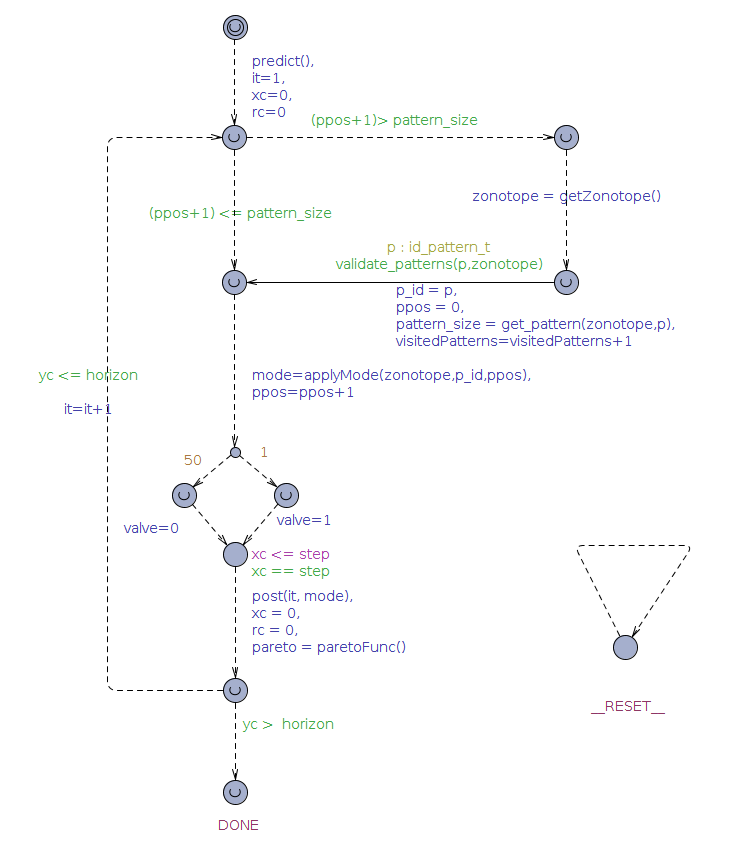
\includegraphics[width=0.7\linewidth]{images/automaton_uppaal}
        %       \captionof{figure}{Template of the safe an near optimal algorithm}
        %   \end{center}
        %   \label{strategotemplate}
        % \end{minipage}

        \begin{figure}[!hbt]
          \centering
          \tikzset{every picture/.style={line width=0.75pt}} %set default line width to 0.75pt        

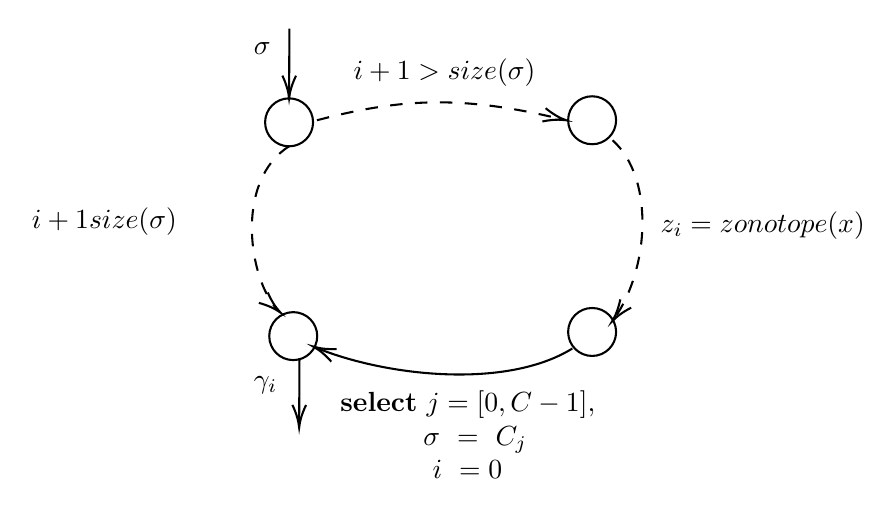
\begin{tikzpicture}[x=0.75pt,y=0.75pt,yscale=-1,xscale=1]
%uncomment if require: \path (0,464); %set diagram left start at 0, and has height of 464

%Shape: Circle [id:dp8712375528286049] 
\draw   (232.89,150.55) .. controls (232.89,144.17) and (238.06,139) .. (244.45,139) .. controls (250.83,139) and (256,144.17) .. (256,150.55) .. controls (256,156.94) and (250.83,162.11) .. (244.45,162.11) .. controls (238.06,162.11) and (232.89,156.94) .. (232.89,150.55) -- cycle ;
%Shape: Circle [id:dp0053736784066187315] 
\draw   (378.89,251.55) .. controls (378.89,245.17) and (384.06,240) .. (390.45,240) .. controls (396.83,240) and (402,245.17) .. (402,251.55) .. controls (402,257.94) and (396.83,263.11) .. (390.45,263.11) .. controls (384.06,263.11) and (378.89,257.94) .. (378.89,251.55) -- cycle ;
%Shape: Circle [id:dp7786102631576663] 
\draw   (378.89,149.55) .. controls (378.89,143.17) and (384.06,138) .. (390.45,138) .. controls (396.83,138) and (402,143.17) .. (402,149.55) .. controls (402,155.94) and (396.83,161.11) .. (390.45,161.11) .. controls (384.06,161.11) and (378.89,155.94) .. (378.89,149.55) -- cycle ;
%Curve Lines [id:da06892458990894723] 
\draw  [dash pattern={on 4.5pt off 4.5pt}]  (257.89,149.55) .. controls (299.47,138.66) and (328.31,137.57) .. (376.43,149.2) ;
\draw [shift={(377.89,149.55)}, rotate = 193.76] [color={rgb, 255:red, 0; green, 0; blue, 0 }  ][line width=0.75]    (10.93,-3.29) .. controls (6.95,-1.4) and (3.31,-0.3) .. (0,0) .. controls (3.31,0.3) and (6.95,1.4) .. (10.93,3.29)   ;
%Curve Lines [id:da34373825883144815] 
\draw  [dash pattern={on 4.5pt off 4.5pt}]  (244.45,162.11) .. controls (218.1,178.69) and (224.84,226.23) .. (238.96,240.93) ;
\draw [shift={(240.29,242.2)}, rotate = 220.91] [color={rgb, 255:red, 0; green, 0; blue, 0 }  ][line width=0.75]    (10.93,-3.29) .. controls (6.95,-1.4) and (3.31,-0.3) .. (0,0) .. controls (3.31,0.3) and (6.95,1.4) .. (10.93,3.29)   ;
%Curve Lines [id:da0893746859182114] 
\draw  [dash pattern={on 4.5pt off 4.5pt}]  (400.29,159.2) .. controls (420.72,177.37) and (417.97,221.4) .. (401.05,245.13) ;
\draw [shift={(400,246.55)}, rotate = 307.39] [color={rgb, 255:red, 0; green, 0; blue, 0 }  ][line width=0.75]    (10.93,-3.29) .. controls (6.95,-1.4) and (3.31,-0.3) .. (0,0) .. controls (3.31,0.3) and (6.95,1.4) .. (10.93,3.29)   ;
%Shape: Circle [id:dp610189050328179] 
\draw   (234.89,253.55) .. controls (234.89,247.17) and (240.06,242) .. (246.45,242) .. controls (252.83,242) and (258,247.17) .. (258,253.55) .. controls (258,259.94) and (252.83,265.11) .. (246.45,265.11) .. controls (240.06,265.11) and (234.89,259.94) .. (234.89,253.55) -- cycle ;
%Curve Lines [id:da6066202102744167] 
\draw    (380.89,259.55) .. controls (348.78,279.35) and (291.05,272.86) .. (257.52,259.18) ;
\draw [shift={(256,258.55)}, rotate = 382.95] [color={rgb, 255:red, 0; green, 0; blue, 0 }  ][line width=0.75]    (10.93,-3.29) .. controls (6.95,-1.4) and (3.31,-0.3) .. (0,0) .. controls (3.31,0.3) and (6.95,1.4) .. (10.93,3.29)   ;
%Straight Lines [id:da9519097834156862] 
\draw    (249.45,264.11) -- (249.3,295.65) ;
\draw [shift={(249.29,297.65)}, rotate = 270.27] [color={rgb, 255:red, 0; green, 0; blue, 0 }  ][line width=0.75]    (10.93,-3.29) .. controls (6.95,-1.4) and (3.31,-0.3) .. (0,0) .. controls (3.31,0.3) and (6.95,1.4) .. (10.93,3.29)   ;
%Straight Lines [id:da75432083913083] 
\draw    (244.6,105.45) -- (244.46,137) ;
\draw [shift={(244.45,139)}, rotate = 270.27] [color={rgb, 255:red, 0; green, 0; blue, 0 }  ][line width=0.75]    (10.93,-3.29) .. controls (6.95,-1.4) and (3.31,-0.3) .. (0,0) .. controls (3.31,0.3) and (6.95,1.4) .. (10.93,3.29)   ;

% Text Node
\draw (422,192.04) node [anchor=north west][inner sep=0.75pt]    {$z_{i} =zonotope( x)$};
% Text Node
\draw (274,118.4) node [anchor=north west][inner sep=0.75pt]    {$i+1 >size( \sigma )$};
% Text Node
\draw (119,190.4) node [anchor=north west][inner sep=0.75pt]    {$i+1\leqslant size( \sigma )$};
% Text Node
\draw (226,110.4) node [anchor=north west][inner sep=0.75pt]    {$\sigma $};
% Text Node
\draw (226,271.4) node [anchor=north west][inner sep=0.75pt]    {$\gamma _{i}$};
% Text Node
\draw (261,277.4) node [anchor=north west][inner sep=0.75pt]    {$ \begin{array}{l}
\mathbf{select} \ j=[ 0,C-1] ,\\
\ \ \ \ \ \ \ \ \ \sigma \ =\ C_{j}\\
\ \ \ \ \ \ \ \ \ \ i\ =0\\
\end{array}$};


\end{tikzpicture}

          \captionsetup{format=hang}
          \caption{The model of the controller. The \textbf{select} statement is a simplification of having a set of edges with one for each value in the select range.}          
          \label{fig:selectoperator}
        \end{figure}

        The first part in the algorithm consist on mapping the current sate to 
        the corresponding pairs such as zonotope and set of patterns, the 
        \emph{select} statement represent a set of edges each of these with its 
        corresponding pattern; the output is the new strategy when a whole modes
        in the current pattern were visited otherwise it just move to next 
        mode, each mode is associated to a configuration $\gamma_i$.

        Subsequently, we define distributions $\delta^k_i$ which estimates
        events in the system as stochastic discrete perturbations, similar to the 
        defined in the real time \ac{MPC} the distributions are composed by 
        3 normal distributions and 1 uniform distribution as described in 
        \autoref{fig:uncontrollable}. It is important to bear in mind,
        the event accumulation which means the number of valves open 
        depending of the probability, after to define the perturbations 
        in the $x_{clock}<P$ we reset the $x_{clock}=0$. Then, we implement
        an \emph{Euler method} to evolve the system each period $P$, this method
        update the state $x$ using the flow function $\mathcal{F}_{c,u}(x(t),d(t))$
        and defined in \autoref{eq:temperature-equation},\autoref{eq:volume-equation},
        \autoref{eq:Energy-equation} respectively, this updating is 
        subject to a cost function defined in \autoref{eq:costfunction}. Finally, 
        We defined another $y_{clock}$ to limit the processing 
        until it reach the horizon $H$.

      
        \begin{figure}[!hbt]
          \centering
          

\tikzset{every picture/.style={line width=0.75pt}} %set default line width to 0.75pt        

\begin{tikzpicture}[x=0.75pt,y=0.75pt,yscale=-1,xscale=1]
%uncomment if require: \path (0,692); %set diagram left start at 0, and has height of 692

%Shape: Circle [id:dp7284696639089192] 
\draw   (250.89,276.15) .. controls (250.89,273.09) and (253.38,270.6) .. (256.45,270.6) .. controls (259.51,270.6) and (262,273.09) .. (262,276.15) .. controls (262,279.22) and (259.51,281.71) .. (256.45,281.71) .. controls (253.38,281.71) and (250.89,279.22) .. (250.89,276.15) -- cycle ;
%Shape: Circle [id:dp7092344590230357] 
\draw   (245.89,357.15) .. controls (245.89,350.77) and (251.06,345.6) .. (257.45,345.6) .. controls (263.83,345.6) and (269,350.77) .. (269,357.15) .. controls (269,363.54) and (263.83,368.71) .. (257.45,368.71) .. controls (251.06,368.71) and (245.89,363.54) .. (245.89,357.15) -- cycle ;
%Straight Lines [id:da95053023471753] 
\draw  [dash pattern={on 4.5pt off 4.5pt}]  (257.45,368.71) -- (257.31,383.25) ;
\draw [shift={(257.29,385.25)}, rotate = 270.54] [color={rgb, 255:red, 0; green, 0; blue, 0 }  ][line width=0.75]    (10.93,-3.29) .. controls (6.95,-1.4) and (3.31,-0.3) .. (0,0) .. controls (3.31,0.3) and (6.95,1.4) .. (10.93,3.29)   ;
%Straight Lines [id:da6246395919086472] 
\draw  [dash pattern={on 4.5pt off 4.5pt}]  (256.6,260) -- (256.53,262.7) -- (256.48,264.76) -- (256.46,268.6) ;
\draw [shift={(256.45,270.6)}, rotate = 270.34] [color={rgb, 255:red, 0; green, 0; blue, 0 }  ][line width=0.75]    (10.93,-3.29) .. controls (6.95,-1.4) and (3.31,-0.3) .. (0,0) .. controls (3.31,0.3) and (6.95,1.4) .. (10.93,3.29)   ;
%Shape: Circle [id:dp603073223077478] 
\draw   (211,310.65) .. controls (211,304.61) and (215.9,299.71) .. (221.95,299.71) .. controls (227.99,299.71) and (232.89,304.61) .. (232.89,310.65) .. controls (232.89,316.7) and (227.99,321.6) .. (221.95,321.6) .. controls (215.9,321.6) and (211,316.7) .. (211,310.65) -- cycle ;
%Shape: Circle [id:dp929274482174262] 
\draw   (277,310.65) .. controls (277,304.61) and (281.9,299.71) .. (287.95,299.71) .. controls (293.99,299.71) and (298.89,304.61) .. (298.89,310.65) .. controls (298.89,316.7) and (293.99,321.6) .. (287.95,321.6) .. controls (281.9,321.6) and (277,316.7) .. (277,310.65) -- cycle ;
%Straight Lines [id:da4723956433829293] 
\draw  [dash pattern={on 4.5pt off 4.5pt}]  (229.4,319.76) -- (255.98,344.24) ;
\draw [shift={(257.45,345.6)}, rotate = 222.65] [color={rgb, 255:red, 0; green, 0; blue, 0 }  ][line width=0.75]    (10.93,-3.29) .. controls (6.95,-1.4) and (3.31,-0.3) .. (0,0) .. controls (3.31,0.3) and (6.95,1.4) .. (10.93,3.29)   ;
%Straight Lines [id:da5493223449601987] 
\draw  [dash pattern={on 4.5pt off 4.5pt}]  (260.45,278.15) -- (280.95,298.16) ;
\draw [shift={(282.38,299.56)}, rotate = 224.3] [color={rgb, 255:red, 0; green, 0; blue, 0 }  ][line width=0.75]    (10.93,-3.29) .. controls (6.95,-1.4) and (3.31,-0.3) .. (0,0) .. controls (3.31,0.3) and (6.95,1.4) .. (10.93,3.29)   ;
%Straight Lines [id:da4708123952991736] 
\draw  [dash pattern={on 4.5pt off 4.5pt}]  (251.89,278.15) -- (228.9,298.44) ;
\draw [shift={(227.4,299.76)}, rotate = 318.58] [color={rgb, 255:red, 0; green, 0; blue, 0 }  ][line width=0.75]    (10.93,-3.29) .. controls (6.95,-1.4) and (3.31,-0.3) .. (0,0) .. controls (3.31,0.3) and (6.95,1.4) .. (10.93,3.29)   ;
%Shape: Circle [id:dp6748222746281551] 
\draw   (248.89,250.36) .. controls (248.89,245.8) and (252.59,242.11) .. (257.15,242.11) .. controls (261.71,242.11) and (265.4,245.8) .. (265.4,250.36) .. controls (265.4,254.92) and (261.71,258.61) .. (257.15,258.61) .. controls (252.59,258.61) and (248.89,254.92) .. (248.89,250.36) -- cycle ;
%Curve Lines [id:da3847758460174753] 
\draw  [dash pattern={on 4.5pt off 4.5pt}]  (252.4,367.76) .. controls (201.97,421.15) and (176.4,351.76) .. (179.4,303.76) .. controls (182.37,256.24) and (186.61,237.39) .. (247.05,249.97) ;
\draw [shift={(248.89,250.36)}, rotate = 192.11] [color={rgb, 255:red, 0; green, 0; blue, 0 }  ][line width=0.75]    (10.93,-3.29) .. controls (6.95,-1.4) and (3.31,-0.3) .. (0,0) .. controls (3.31,0.3) and (6.95,1.4) .. (10.93,3.29)   ;
%Shape: Circle [id:dp48342387303657786] 
\draw   (246.34,395.31) .. controls (246.34,389.26) and (251.24,384.36) .. (257.29,384.36) .. controls (263.34,384.36) and (268.24,389.26) .. (268.24,395.31) .. controls (268.24,401.35) and (263.34,406.25) .. (257.29,406.25) .. controls (251.24,406.25) and (246.34,401.35) .. (246.34,395.31) -- cycle ;
%Straight Lines [id:da7144351519944012] 
\draw  [dash pattern={on 4.5pt off 4.5pt}]  (257.29,413.25) -- (257.22,427.9) -- (258.26,490.71) ;
\draw [shift={(258.29,492.71)}, rotate = 269.06] [color={rgb, 255:red, 0; green, 0; blue, 0 }  ][line width=0.75]    (10.93,-3.29) .. controls (6.95,-1.4) and (3.31,-0.3) .. (0,0) .. controls (3.31,0.3) and (6.95,1.4) .. (10.93,3.29)   ;
%Shape: Circle [id:dp7106124708128221] 
\draw   (247.34,503.65) .. controls (247.34,497.61) and (252.24,492.71) .. (258.29,492.71) .. controls (264.34,492.71) and (269.24,497.61) .. (269.24,503.65) .. controls (269.24,509.7) and (264.34,514.6) .. (258.29,514.6) .. controls (252.24,514.6) and (247.34,509.7) .. (247.34,503.65) -- cycle ;
%Straight Lines [id:da6141215757734786] 
\draw  [dash pattern={on 4.5pt off 4.5pt}]  (258.29,514.6) -- (258.14,542.15) ;
\draw [shift={(258.13,544.15)}, rotate = 270.3] [color={rgb, 255:red, 0; green, 0; blue, 0 }  ][line width=0.75]    (10.93,-3.29) .. controls (6.95,-1.4) and (3.31,-0.3) .. (0,0) .. controls (3.31,0.3) and (6.95,1.4) .. (10.93,3.29)   ;
%Curve Lines [id:da15340003106255407] 
\draw  [dash pattern={on 4.5pt off 4.5pt}]  (258.29,514.6) .. controls (112.4,679.76) and (50.4,-20.24) .. (248.62,113.41) ;
\draw [shift={(248.62,113.41)}, rotate = 213.99] [color={rgb, 255:red, 0; green, 0; blue, 0 }  ][line width=0.75]    (10.93,-3.29) .. controls (6.95,-1.4) and (3.31,-0.3) .. (0,0) .. controls (3.31,0.3) and (6.95,1.4) .. (10.93,3.29)   ;
%Straight Lines [id:da7413495490612987] 
\draw  [dash pattern={on 4.5pt off 4.5pt}]  (281.4,319.76) -- (258.81,344.13) ;
\draw [shift={(257.45,345.6)}, rotate = 312.83] [color={rgb, 255:red, 0; green, 0; blue, 0 }  ][line width=0.75]    (10.93,-3.29) .. controls (6.95,-1.4) and (3.31,-0.3) .. (0,0) .. controls (3.31,0.3) and (6.95,1.4) .. (10.93,3.29)   ;
%Shape: Ellipse [id:dp3588768055128455] 
\draw   (248.62,113.41) .. controls (248.62,108.51) and (252.25,104.53) .. (256.72,104.53) .. controls (261.2,104.53) and (264.83,108.51) .. (264.83,113.41) .. controls (264.83,118.31) and (261.2,122.28) .. (256.72,122.28) .. controls (252.25,122.28) and (248.62,118.31) .. (248.62,113.41) -- cycle ;
%Shape: Ellipse [id:dp3302959902263827] 
\draw   (364.06,192) .. controls (364.06,187.09) and (367.69,183.12) .. (372.17,183.12) .. controls (376.64,183.12) and (380.27,187.09) .. (380.27,192) .. controls (380.27,196.9) and (376.64,200.87) .. (372.17,200.87) .. controls (367.69,200.87) and (364.06,196.9) .. (364.06,192) -- cycle ;
%Shape: Ellipse [id:dp2177769209104332] 
\draw   (363.06,114.64) .. controls (363.06,109.74) and (366.69,105.76) .. (371.17,105.76) .. controls (375.64,105.76) and (379.27,109.74) .. (379.27,114.64) .. controls (379.27,119.54) and (375.64,123.52) .. (371.17,123.52) .. controls (366.69,123.52) and (363.06,119.54) .. (363.06,114.64) -- cycle ;
%Curve Lines [id:da43407130814922046] 
\draw  [dash pattern={on 4.5pt off 4.5pt}]  (266.16,112.64) .. controls (295.18,104.32) and (327.69,105.39) .. (361.51,114.23) ;
\draw [shift={(363.06,114.64)}, rotate = 195.01] [color={rgb, 255:red, 0; green, 0; blue, 0 }  ][line width=0.75]    (10.93,-3.29) .. controls (6.95,-1.4) and (3.31,-0.3) .. (0,0) .. controls (3.31,0.3) and (6.95,1.4) .. (10.93,3.29)   ;
%Curve Lines [id:da9780706925040288] 
\draw  [dash pattern={on 4.5pt off 4.5pt}]  (251.81,121.52) .. controls (244.7,129.43) and (243.38,170.36) .. (252.6,182.45) ;
\draw [shift={(253.81,183.81)}, rotate = 223.5] [color={rgb, 255:red, 0; green, 0; blue, 0 }  ][line width=0.75]    (10.93,-3.29) .. controls (6.95,-1.4) and (3.31,-0.3) .. (0,0) .. controls (3.31,0.3) and (6.95,1.4) .. (10.93,3.29)   ;
%Curve Lines [id:da3797599022693716] 
\draw  [dash pattern={on 4.5pt off 4.5pt}]  (377.07,123.05) .. controls (391.26,136.87) and (388.57,164.5) .. (376.97,182.51) ;
\draw [shift={(375.87,184.16)}, rotate = 304.92] [color={rgb, 255:red, 0; green, 0; blue, 0 }  ][line width=0.75]    (10.93,-3.29) .. controls (6.95,-1.4) and (3.31,-0.3) .. (0,0) .. controls (3.31,0.3) and (6.95,1.4) .. (10.93,3.29)   ;
%Shape: Ellipse [id:dp36872861031148263] 
\draw   (250.02,192.53) .. controls (250.02,187.63) and (253.65,183.66) .. (258.13,183.66) .. controls (262.6,183.66) and (266.23,187.63) .. (266.23,192.53) .. controls (266.23,197.43) and (262.6,201.41) .. (258.13,201.41) .. controls (253.65,201.41) and (250.02,197.43) .. (250.02,192.53) -- cycle ;
%Curve Lines [id:da896328789252695] 
\draw    (365.4,197.76) .. controls (340.05,207.51) and (293.02,209.28) .. (269.03,199.32) ;
\draw [shift={(267.23,198.53)}, rotate = 24.88] [color={rgb, 255:red, 0; green, 0; blue, 0 }  ][line width=0.75]    (10.93,-3.29) .. controls (6.95,-1.4) and (3.31,-0.3) .. (0,0) .. controls (3.31,0.3) and (6.95,1.4) .. (10.93,3.29)   ;
%Straight Lines [id:da0980624263296852] 
\draw    (256.83,78.76) -- (256.73,102.53) ;
\draw [shift={(256.72,104.53)}, rotate = 270.24] [color={rgb, 255:red, 0; green, 0; blue, 0 }  ][line width=0.75]    (10.93,-3.29) .. controls (6.95,-1.4) and (3.31,-0.3) .. (0,0) .. controls (3.31,0.3) and (6.95,1.4) .. (10.93,3.29)   ;
%Straight Lines [id:da3888311958049726] 
\draw  [dash pattern={on 4.5pt off 4.5pt}]  (257.13,202.41) -- (256.98,238.95) ;
\draw [shift={(256.97,240.95)}, rotate = 270.23] [color={rgb, 255:red, 0; green, 0; blue, 0 }  ][line width=0.75]    (10.93,-3.29) .. controls (6.95,-1.4) and (3.31,-0.3) .. (0,0) .. controls (3.31,0.3) and (6.95,1.4) .. (10.93,3.29)   ;

% Text Node
\draw (183,168) node [anchor=north west][inner sep=0.75pt]  [font=\small]  {$ \begin{array}{l}
\ \ \ \ \ \ \ \ \ \ \gamma _{i} ,\\
i\leftarrow i+1\\
\ \ \ \ \ v\leftarrow 0\\
\ \ \ \ \ k\leftarrow 0
\end{array}$};
% Text Node
\draw (275,270) node [anchor=north west][inner sep=0.75pt]    {$\delta _{i}^{k}\textcolor[rgb]{0.29,0.56,0.89}{.....................................}( a)$};
% Text Node
\draw (195,269) node [anchor=north west][inner sep=0.75pt]    {$1-\delta _{i}^{k}$};
% Text Node
\draw (280,323) node [anchor=north west][inner sep=0.75pt]    {$v\leftarrow v+1\textcolor[rgb]{0.29,0.56,0.89}{\ ......................}( b)$};
% Text Node
\draw (136,303) node [anchor=north west][inner sep=0.75pt]    {$ \begin{array}{l}
k\leftarrow k+1\\
\ \ \ \ \ \ \ k\leqslant 3
\end{array}$};
% Text Node
\draw (273,349) node [anchor=north west][inner sep=0.75pt]    {$k >3$};
% Text Node
\draw (270.24,385.71) node [anchor=north west][inner sep=0.75pt]    {$x_{Clock} \leqslant step$};
% Text Node
\draw (266.22,483.3) node [anchor=north west][inner sep=0.75pt]    {$x_{Clock}\leftarrow 0$};
% Text Node
\draw (267,430) node [anchor=north west][inner sep=0.75pt]    {$\sigma _{opt} =\underset{\underset{}{\sigma \subseteq \sigma _{safe}}}{\text{argmin}} \ ( \alpha E+( 1-\alpha )( T-T_{g}))$};
% Text Node
\draw (267,408) node [anchor=north west][inner sep=0.75pt]    {$x=\mathcal{F}_{c,u}( \tau ,x,d) \ \textcolor[rgb]{0.29,0.56,0.89}{..............} \ ( c)$};
% Text Node
\draw (271,522) node [anchor=north west][inner sep=0.75pt]    {$y_{Clock}  >H$};
% Text Node
\draw (45,317) node [anchor=north west][inner sep=0.75pt]    {$y_{Clock} \leqslant H$};
% Text Node
\draw (394,143.28) node [anchor=north west][inner sep=0.75pt]    {$z_{i} =zonotope( x)$};
% Text Node
\draw (144.49,145.26) node [anchor=north west][inner sep=0.75pt]    {$i+1\leqslant size( \sigma )$};
% Text Node
\draw (241.84,73.8) node [anchor=north west][inner sep=0.75pt]    {$\sigma $};
% Text Node
\draw (269.41,211.9) node [anchor=north west][inner sep=0.75pt]  [font=\small]  {$ \begin{array}{l}
\mathbf{select} \ j=[ 0,C-1] ,\\
\ \ \ \ \ \ \ \ \ \sigma \ =\ C_{j}\\
\ \ \ \ \ \ \ \ \ \ i\ =0\\
\end{array}$};
% Text Node
\draw (272,85.4) node [anchor=north west][inner sep=0.75pt]    {$i+1 >size( \sigma )$};
% Text Node
\draw (510,288.4) node [anchor=north west][inner sep=0.75pt]  [font=\footnotesize]  {$ \begin{array}{l}
Uncontrollable\\
\ computation
\end{array}$};
% Text Node
\draw (508,454.4) node [anchor=north west][inner sep=0.75pt]  [font=\footnotesize]  {$ \begin{array}{l}
Controllable\\
\ computation
\end{array}$};
% Text Node
\draw (265,466) node [anchor=north west][inner sep=0.75pt]    {$c'=\sigma _{opt}( \gamma _{i}) ,\ u'=v\ \textcolor[rgb]{0.29,0.56,0.89}{.......} \ ( d)$};
% Text Node
\draw (263.15,258.01) node [anchor=north west][inner sep=0.75pt]    {$u$};
% Text Node
\draw (300.15,301.01) node [anchor=north west][inner sep=0.75pt]    {$u'$};


\end{tikzpicture}

          \captionsetup{format=hang}
          \caption{The model generating stochastic perturbations as valve aperturing and closing}
          \label{fig:perturbationsgeneration}
        \end{figure}
        

        \clearpage

        After to define the automaton as \ac{SHG} \textsc{Uppaal Stratego}
        we use the command 1 to find the strategy which minimize the cost 
        function in a horizon $H$. Then, simulate the system for a horizon
        in order to get modes. These modes are used in the real time 
        simulator which use \ac{MPC} to optimize strategies subject to safe
        patterns for $24h$ as shown in \autoref{fig:resulta}.

        \begin{lstlisting}
          1. strategy Opt = minE (pareto) [<=horizon]: 
          <> GTime>=horizon
          2. simulate 1 [<=horizon] {mode} under Opt
        \end{lstlisting}

        We notice a better performace with online control using \textsc{stratego}
        because  of the stochastic aproach which explore the best set of modes in 
        a \emph{horizon} $H$ \textsc{stratego} not only verify the system correcteness
        but also explore strategies which optimize the cost function, which include
        the energy consumption and temperature distance.
        \begin{figure}[!htb]        
          \begin{subfigure}{0.51\textwidth}
            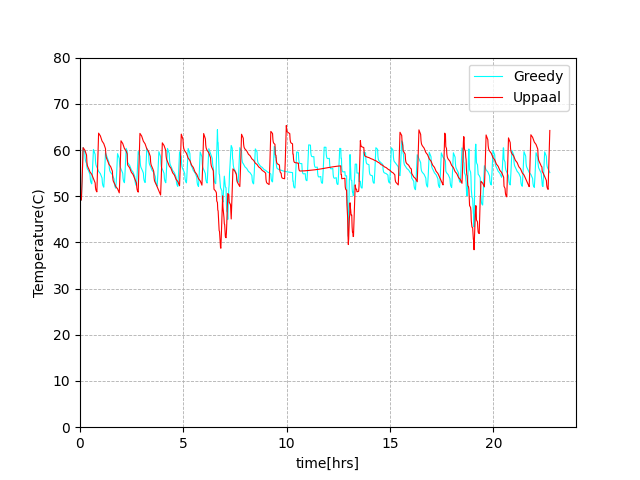
\includegraphics[width=1.0\linewidth]{images/controllers1.png}
            \captionsetup{format=hang}
            \captionof{figure}{Temperatures responses from greedy and 
            reinforcement learning optimizations, both using safe patterns.} \label{fig:resulta}
          \end{subfigure}
          \hspace*{\fill}
          \begin{subfigure}{0.51\textwidth}
              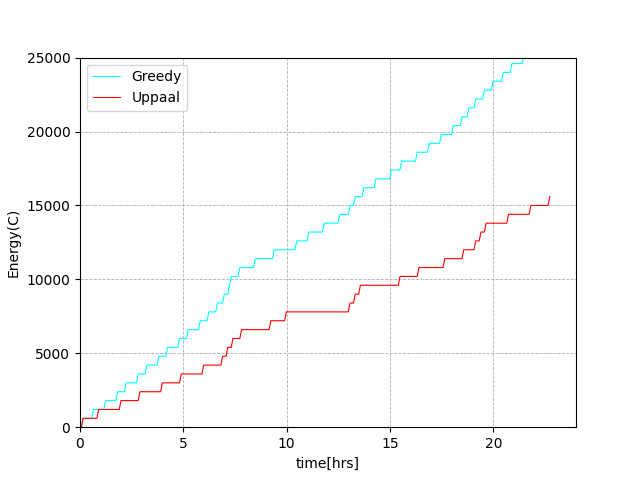
\includegraphics[width=1.0\linewidth]{images/energycomparison.png}
              \captionsetup{format=hang}
              \caption{Energy consumption comparison between greedy and reinforcement
              learning trough \textsc{Uppaal}, both using safe patterns.} \label{fig:resultb}
          \end{subfigure}%            
          \caption{Solar water heating 24h trajectories of two control strategies}
        \end{figure}

      For $\alpha = 0.5$ defined in \autoref{eq:costfunction} that means we assign the same 
      importance to the temperatures distance and the energy consumption saving in the 
      optimization, the mean temperature error in the greedy method 
      \autoref{fig:resulta} is : $2.07$ and the reinforcement learning optimization 
      is:  $3.42$ and also the saved energy consumption using uppaal with respect to 
      a greedy method is $ S = \bigtriangleup E_{greedy} - \bigtriangleup E_{uppaal} = 10800.0Kw$
       as \autoref{fig:resultb} shows. % 310800.0
        
          % \textbf{Evaluation Scenarios}
          % \textbf{Controller Evaluation}
